\documentclass{report}

\usepackage[utf8]{inputenc} % Charakter-Kodierung
\usepackage[german]{babel} % Sprache

\usepackage[table,xcdraw]{xcolor} % Tabellen Farben
\usepackage{tabularx} % Dynamische Tabellenbreite
\usepackage{tcolorbox} % Graue Boxen
\usepackage{hyperref} % url Umgebung
\usepackage{todonotes} % Notizen
\usepackage{natbib} % Bibliographie
\usepackage{fancyhdr} % Header und Footer
\usepackage{multirow} % Multizeile
\usepackage{geometry} % Page layout
\usepackage{color} % Text Farben
\usepackage{float}

% Page layout
\geometry{
	bottom=3.5cm,
	headheight=180pt
}

% Nummerierung der ersten Seiten verhindern
\pagenumbering{gobble}

% Bibstyle
\bibliographystyle{plain}

% Header / Footer
\fancypagestyle{plain}{
	\fancyhf{}% Clear header/footer
	\fancyhead[R]{
\includegraphics[width=4cm]{img/cau-logo-2017}} % Rechter header
	\fancyhead[L]{\leftmark} % Linker header
	\fancyfoot[R]{\thepage} % Rechter footer
	\fancyfoot[L]{
\includegraphics[width=1cm]{img/se-logo}} % Linker footer	
}
\pagestyle{plain}

\renewcommand{\headrulewidth}{0.5pt} % Unnötige Informationen der Kapitelangabe
\renewcommand{\footrulewidth}{0.2pt} % entfernen
\renewcommand{\chaptermark}[1]{\markboth{{#1}}{}}




% Zahlen für Fußnoten
\renewcommand{\thefootnote}{\arabic{footnote}}
\renewcommand{\thempfootnote}{\arabic{mpfootnote}}

%%%%% Ausfüllen %%%%%

% Gruppenname
\newcommand{\gruppenname}{Gruppe LMS8 EG 016}

% Projektname
\newcommand{\projektname}{VOTEsso}

% Semester
\newcommand{\semester}{Sommer 2022}



% Titelseite

\title{
	\vspace*{-5cm}
	Entwurfsdokumentation\\
	\textbf \projektname\\
	Bürgerbeteiligung Kiel\\
	-\\
	\color{gray}
	Softwareprojekt \semester\\
	\gruppenname\\
	\vspace*{5mm}
	
\includegraphics[width=\textwidth]{img/logo}
}

\author{
	\begin{tabular}{r l@{\hspace{8\tabcolsep}} r} 
		Heiko & Bielfeldt & \multirow{8}{*}{ 
\includegraphics{img/se-logo} } \\
		Markus & Glaubitz \\
		Niclas & Nebelung \\
		Sören & Petersen \\
		Arne & Seufert \\
		Jonas & Struve \\
		Jon & Stührwoldt \\
		Arne & Wiese \\
	\end{tabular}
}

\date{\today}





% Dokument

\begin{document}
	\maketitle
	
	\tableofcontents 
	
	\chapter{Einleitung}\label{chp:einleitung}
	\pagenumbering{arabic} % Nummerierung starten
	\thispagestyle{fancy}
	Nachdem die Anforderungen an die Software, das Anwendungsgebiet und die Zielgruppe bestimmt wurden, wird nun ein abstrakteres (und deutlich technischeres) Modell dokumentiert. Die nach dem Pflichtenheft zu erstellende Entwurfsdokumententation  legt technische Spezifikationen des zukünfigten Systems der Software fest.

In dieser Phase der Dokumentation sollen erste Nachweise geschaffen werden, die die technische Umsetzbarkeit des Systems
und die richtige Funktionsweise zeigen. Wichtig ist hierbei zu beachten, dass es sich um einen ersten Entwurf der Software nach jetzigem Verständnis der verwendeten Technologien und Systemumgebung handelt. Während der Softwareentwicklung werden sich Teile des Systementwurfs nach Notwendigkeiten ändern. Dies wird seperat dokumentiert.\\


Hier wird versucht die realen Anforderungen in technischer Hinsicht abzubilden.
Im Vordergrund steht die Transparenz der Systemarchitektur durch die Abbildung wichtiger Prozesse und Interaktionen zwischen Systemteilen.
Um eine möglichst genauen und verständlichen Überblick zu schaffen, werden hier einige verschiedene Diagrammarten, welche sich an der UML orientieren, verwendet:\\
Der Einsatz von Hardware und die dort eingesetzten Softwareumgebungen zur Ausführung der Systemteile sind in Verteilungsdiagrammen zu erkennen.\\
Eine kompaktere und weniger detailtierte Ansicht des Systems sind in Komponentendiagrammen zu finden, in denen auch externe Anbindungen realisiert sind.\\
Sinn der Klassendiagramme ist unter anderem die Zusammenhänge von Klassen und Komponenten darzustellen und die Komplexität dieser gezielt zum Beispiel durch
Modularisierung zu reduzieren.\\
Um die Abläufe und Kommunikation zwischen Komponenten und Klassen zur Laufzeit darzustellen, werden Sequenzdiagramme verwendet.\\
\begin{tcolorbox}
Die Diagramme sind nochmal separat in einem Unterordner (als Vektorgrafik) zu finden, da sie zum Teil komplex und recht groß ausfallen und möglicherweise in diesem Dokument schwer zu lesen sind.
\end{tcolorbox}

\newpage
\section{Entwicklungsumgebung}\label{sec:entwicklungsumgebung}

\begin{table}[h]
	\centering
	\begin{tabularx}{\textwidth}{l l X}
		\rowcolor[HTML]{C0C0C0} 
		\textbf{Software} & \textbf{Version} & \textbf{URL} \\
		Java Development Kit & 17.0.1 & \url{http://www.oracle.com/technetwork/java/javase/downloads/index.html} \\
		\rowcolor[HTML]{E7E7E7} 
		Android Studio Chipmunk & 2021.2.1 (Patch 2) & \url{https://developer.android.com/studio} \\
		Android & 11 & \url{https://developer.android.com/about/versions/11/} \\
		\rowcolor[HTML]{E7E7E7} 
		Spring Boot & 2.7.0 & \url{https://spring.io/} \\
		Thymeleaf & von Spring eingebunden & \url{https://www.thymeleaf.org/} \\
		\rowcolor[HTML]{E7E7E7} 
		Bootstrap & von Spring eingebunden & \url{https://getbootstrap.com/} \\
		Lombok & 6.4.3 & \url{https://projectlombok.org/} \\
		\rowcolor[HTML]{E7E7E7} 
		Gradle & 7.5.1 & \url{https://gradle.org/} \\
		Docker & 20.10.17 & \url{https://www.docker.com/} \\
		\rowcolor[HTML]{E7E7E7} 
		Git & 2.37.3 & \url{https://git-scm.com/} \\
		Retrofit & 2.9.0 & \url{https://square.github.io/retrofit/} \\
		\rowcolor[HTML]{E7E7E7} 
		PostgreSQL & 9.6.21  & \url{https://www.postgresql.org/}\\
	\end{tabularx}
	\caption{Enwicklungsumgebung}
	\label{table:entwicklungsumgebung}
\end{table}

	
	\chapter{Team-Aufteilung}
	\thispagestyle{fancy}
	\begin{tabular}{ll}
 \rowcolor[HTML]{E7E7E7} 
 \textbf{Name} & \textbf{Zuständigkeit} \\ \hline
 Markus Glaubitz & App \\ 
 \rowcolor[HTML]{E7E7E7} 
 Niclas Nebelung & App \\ 
 Sören Petersen & App \\ 
 \rowcolor[HTML]{E7E7E7} 
 Arne Seufert & App \\ 
 Heiko Bielfeldt & Frontend Web, Backend \\ 
 \rowcolor[HTML]{E7E7E7}
 Jonas Struve &  Backend \\ 
 Jon Stührwoldt & Backend \\ 
 \rowcolor[HTML]{E7E7E7}
 Arne Wiese & Backend \\ 
\end{tabular}

\bigskip

Aufgrund des derzeitigen Projektfortschrittes ist bis jetzt noch keine genauere Aufgabenteilung erfolgt. Diese wird in der Entwicklungszeit dynamisch stattfinden.\\
	
	\chapter{Komponentendiagramme}\label{chp:komponentendiagramme}
	\thispagestyle{fancy}
	\section{Komponentendiagramm Web}

\begin{figure}[H]
	\centering
	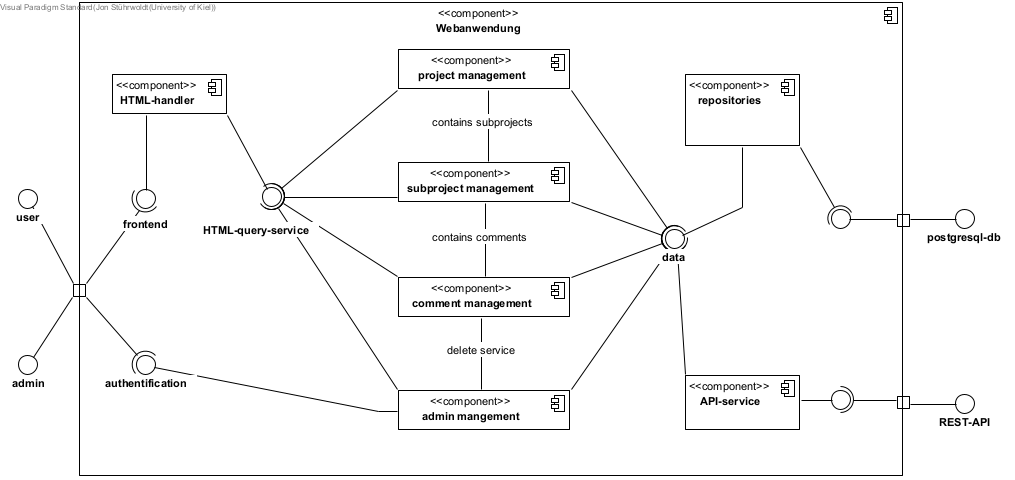
\includegraphics[width=\textwidth]{img/componentweb.png}	
	\caption{Komponentendiagramm - Web}
	\label{fig:komponentendiagramm-a}
\end{figure}

\begin{table}[H]
	\centering
	\begin{tabularx}{\textwidth}{X X}
		\rowcolor[HTML]{C0C0C0} 
		\textbf{Subkomponente} & \textbf{Aufgabe} \\
		HTML-handler & Verwaltet und erstellt HTML-Dokumente und deren Inhalt. \\
		\rowcolor[HTML]{E7E7E7}
		project management & Ruft Daten für Projekte auf und stellt sie dem jeweiligen HTML-Dokument bereit.   \\
		 subproject management &  Ruft Daten für Teilprojekte auf und stellt sie dem jeweiligen HTML-Dokument bereit. \\
		 \rowcolor[HTML]{E7E7E7}
		comment management & Ruft Daten für Kommentare auf und stellt sie dem jeweiligen HTML-Dokument (Detailübersicht eines Teilprojekts) bereit. Verwaltet des Weiteren den Löschvorgang von Kommentaren für Administratoren. \\
		admin management & Ruft Daten für die Anmeldung als Administrator auf und stellt sie dem jeweiligen HTML-Dokument bereit. Verwaltet außerdem die Autorisierung zum Löschen von Kommentaren.   \\
		\rowcolor[HTML]{E7E7E7}
		repositories & Stellt den angefragten Datenbestand der PostgreSQL-Datenbank bereit und ist zentral für die nachträgliche Aktualisierung der Daten im Falle einer Änderung (z.B. Kommentar erstellen oder löschen). \\
		API-services & Verwaltet den Datenfluss zwischen Backend und App. \\
		
	\end{tabularx}
	\caption{Komponentenbeschreibung - Web}
	\label{table:komponentenbeschreibung-web}
\end{table}


\section{Komponentendiagramm App}

\begin{figure}[H]
	\centering
	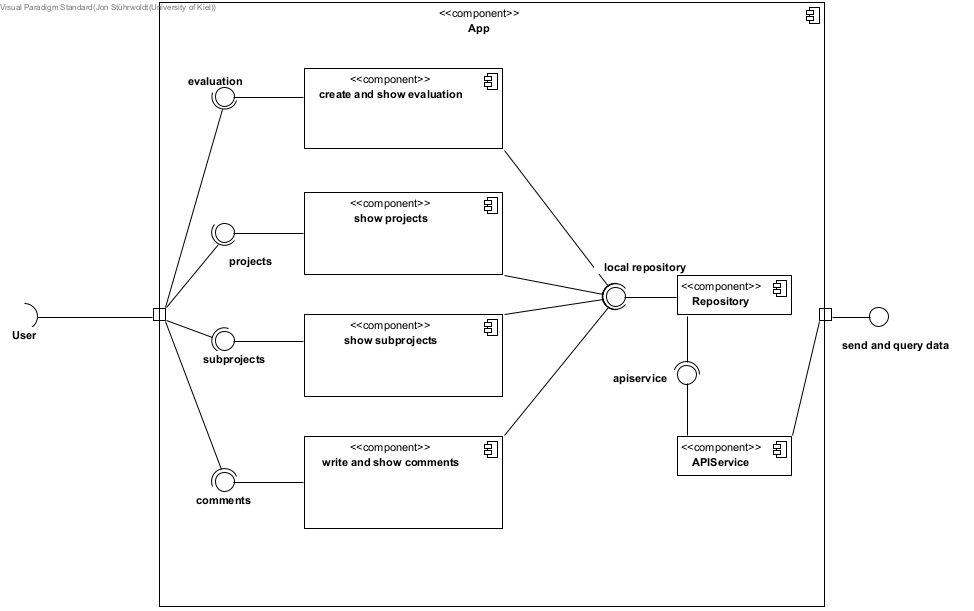
\includegraphics[width=\textwidth]{img/componentapp.png}	
	\caption{Komponentendiagramm - App}
	\label{fig:komponentendiagramm-b}
\end{figure}

\begin{table}[H]
	\centering
	\begin{tabularx}{\textwidth}{X X}
		\rowcolor[HTML]{C0C0C0} 
		\textbf{Subkomponente} & \textbf{Aufgabe} \\
		write and show comments & Diese Komponente ermöglicht es dem User zu vorher ausgewählten Teilprojekten einen für alle anderen User sichtbaren Kommentar abzugeben oder Kommentare von anderen Usern anzuschauen. \\
		\rowcolor[HTML]{E7E7E7}
		create and show evaluation & Diese Komponente bietet dem User die Möglichkeit eine Bewertung in Form von Daumen hoch oder Daumen runter abzugeben und die Bewertung anderer User anzuschauen.   \\
		 Repository &  Diese Komponente speichert die benötigten Daten zur Laufzeit und stellt sie den anderen Komponenten zur Verfügung. Außerdem kommuniziert sie mit dem APIService um Daten zu senden und zu empfangen. \\
		 \rowcolor[HTML]{E7E7E7}
		show projects & In dieser Komponente werden dem User alle verfügbaren Hauptprojekte angezeigt. Außerdem ist sie dafür verantwortlich nach Auswahl eines Hauptprojektes die entsprechende Detailseite anzuzeigen. \\
		show subprojects & In dieser Komponente werden dem User alle zu einem Hauptprojekt zugehörigen Teilprojekte,  nach Entfernung sortiert, angezeigt. Zudem sorgt diese Komponente auch dafür, die entsprechende Teilprojekt Detailseite anzuzeigen.   \\
		\rowcolor[HTML]{E7E7E7}
		APIService & Diese Komponente übernimmt die Kommunikation mit dem Backend. Sie ist sowohl dafür verantwortlich beim Start der App die Daten zu holen, als auch neue Daten zu senden. \\
		API-services & Verwaltet den Datenfluss zwischen Backend und App. \\
		
	\end{tabularx}
	\caption{Komponentenbeschreibung - App}
	\label{table:komponentenbeschreibung-app}
\end{table}
	
	\chapter{Verteilungsdiagramm}\label{chp:verteilungsdiagramm}
	\thispagestyle{fancy}
	Da das zukünftige Deployment des Systems noch durchaus ungewiss ist, ist hier wie abgesprochen das Deployment in der Entwicklungsphase an der CAU dokumentiert.

\begin{figure}[h]
	\centering
	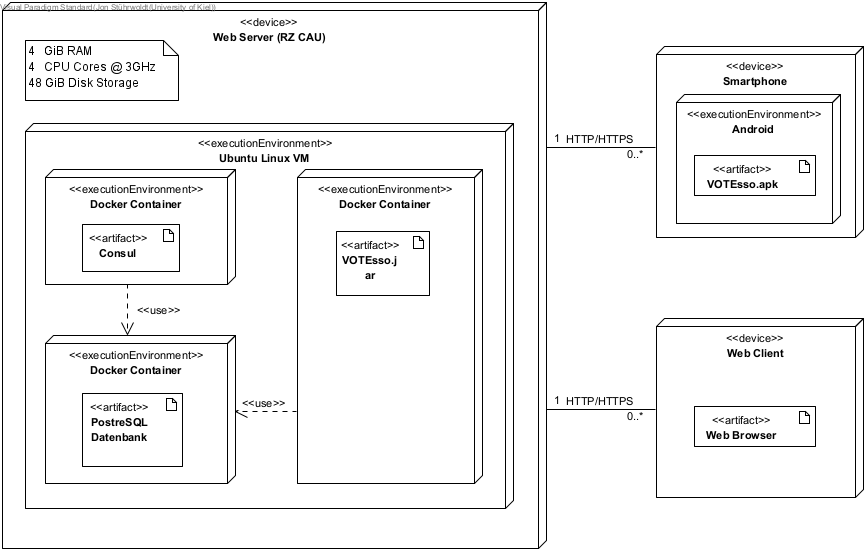
\includegraphics[width=\textwidth]{img/deployment.png}	
	\caption{Verteilungsdiagramm}
	\label{fig:verteilungsdiagramm}
\end{figure}
		
	\chapter{Klassendiagramme}\label{chp:klassendiagramme}
	\thispagestyle{fancy}
	\section{Klassendiagramme Web}
\subsection{VOTEsso und Configurations}
\begin{figure}[htp]
	\centering
	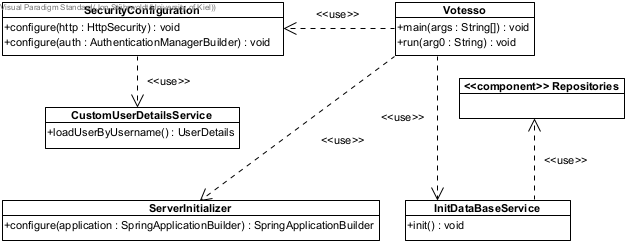
\includegraphics[width=\textwidth]{img/classvotesso.png}	
	\caption{Klassendiagramm - Configurations}
	\label{fig:klassendiagramm-vote}
\end{figure}

\begin{table}[htp]
	\centering
	\begin{tabularx}{\textwidth}{X X}
		\rowcolor[HTML]{C0C0C0} 
		\textbf{Klassenname} & \textbf{Aufgabe} \\
		Votesso & Main-Klasse, über die das Programm gestartet werden kann. \\
		\rowcolor[HTML]{E7E7E7}
		SecurityConfiguration & Verwaltet den Zugriff auf URLs.   \\
		 CustomUserDetailsService &  Kümmert sich um die Autorisierung, beim Login von Administratoren. \\
		 \rowcolor[HTML]{E7E7E7}
		ServerInitializer & Konfiguriert und baut die Anwendung. \\
		InitDataBaseService & Initialisiert alle Repositries mit dem jeweiligen Datenbankinhalt.  \\
	\end{tabularx}
	\caption{Klassenbeschreibung - Web, Configurations}
	\label{table:klassenbeschreibung-web-configurations}
\end{table}


\subsection{Model}
\begin{figure}[H]
	\centering
	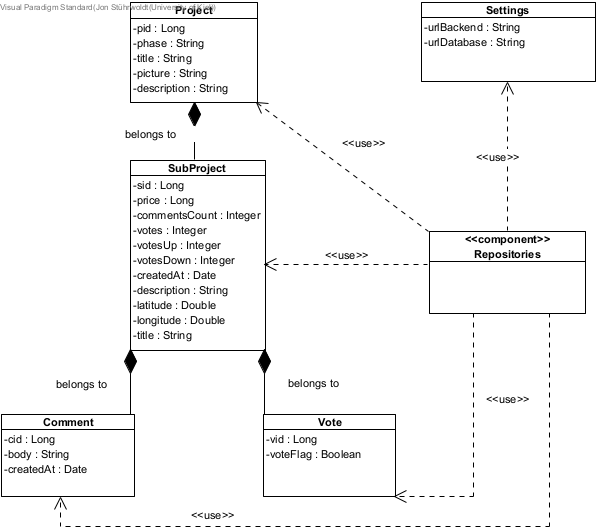
\includegraphics[width=\textwidth]{img/classmodel.png}	
	\caption{Klassendiagramm - Model}
	\label{fig:klassendiagramm-model}
\end{figure}

\begin{table}[H]
	\centering
	\begin{tabularx}{\textwidth}{X X}
		\rowcolor[HTML]{C0C0C0} 
		\textbf{Klassenname} & \textbf{Aufgabe} \\
		Project & Klasse, die den Datentypen Project repräsentiert und alle nötigen Informationen eines (Haupt-)Projekts enthält. Der Aufbau der Klasse dient als Vorlage für die Objekte, die im zugehörigen Repository abgespeichert werden. \\
		\rowcolor[HTML]{E7E7E7} 
		 SubProject &  Klasse, die den Datentypen SubProject repräsentiert und alle nötigen Informationen eines TeilProjekts enthält. Der Aufbau der Klasse dient als Vorlage für die Objekte, die im zugehörigen Repository abgespeichert werden. \\
		Comment & Klasse, die den Datentypen Comment repräsentiert und alle nötigen Informationen eines Kommentars enthält. Der Aufbau der Klasse dient als Vorlage für die Objekte, die im zugehörigen Repository abgespeichert werden. \\
		\rowcolor[HTML]{E7E7E7} 
		Vote & Klasse, die den Datentypen Vote repräsentiert und alle nötigen Informationen einer Abstimmung/Bewertung enthält. Der Aufbau der Klasse dient als Vorlage für die Objekte, die im zugehörigen Repository abgespeichert werden. \\
		Settings & Klasse, die die URLs enthält, welche durch den Administrator konfigurierbar sind. Von dieser Klasse soll später lediglich eine Instanz existieren. Der Aufbau der Klasse dient als Vorlage für das eine Objekt, welches im zugehörigen Repository abgespeichert wird.  \\
	\end{tabularx}
	\caption{Klassenbeschreibung - Web, Model}
	\label{table:klassenbeschreibung-web-model}
\end{table}

\subsection{Repositories}
\begin{figure}[H]
	\centering
	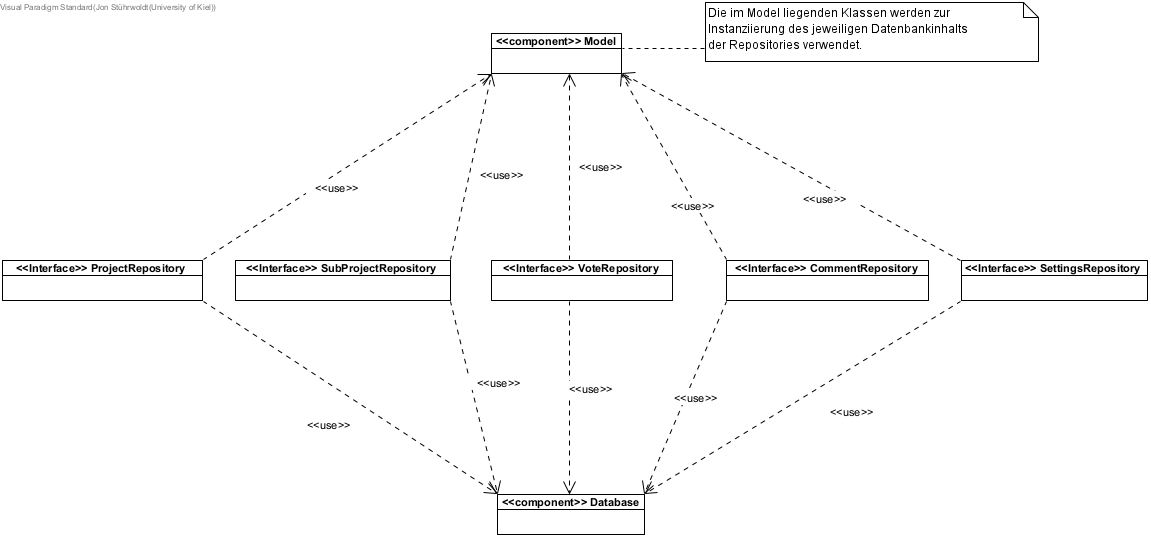
\includegraphics[width=\textwidth]{img/classrepo.png}	
	\caption{Klassendiagramm - Repositories}
	\label{fig:klassendiagramm-repo}
\end{figure}

\begin{table}[H]
	\centering
	\begin{tabularx}{\textwidth}{X X}
		\rowcolor[HTML]{C0C0C0} 
		\textbf{Klassenname} & \textbf{Aufgabe} \\
		ProjectRepository & Interface, welches die Verwaltung von Objekten des Datentyps Project übernimmt. \\
		\rowcolor[HTML]{E7E7E7}
		SubProjectRepository & Interface, welches die Verwaltung von Objekten des Datentyps SubProject übernimmt.  \\
		 VoteRepository &  Interface, welches die Verwaltung von Objekten des Datentyps Vote übernimmt. \\
		 \rowcolor[HTML]{E7E7E7}
		CommentRepository & Interface, welches die Verwaltung von Objekten des Datentyps Comment übernimmt. \\
		SettingsRepository & Interface, welches die Verwaltung der einen Instanz der Klasse Settings übernimmt.  \\
	\end{tabularx}
	\caption{Klassenbeschreibung - Web, Repositories}
	\label{table:klassenbeschreibung-web-repositories}
\end{table}

Die Interfaces werden durch das Spring Boot Framework realisiert.


\subsection{Controller}
\begin{figure}[H]
	\centering
	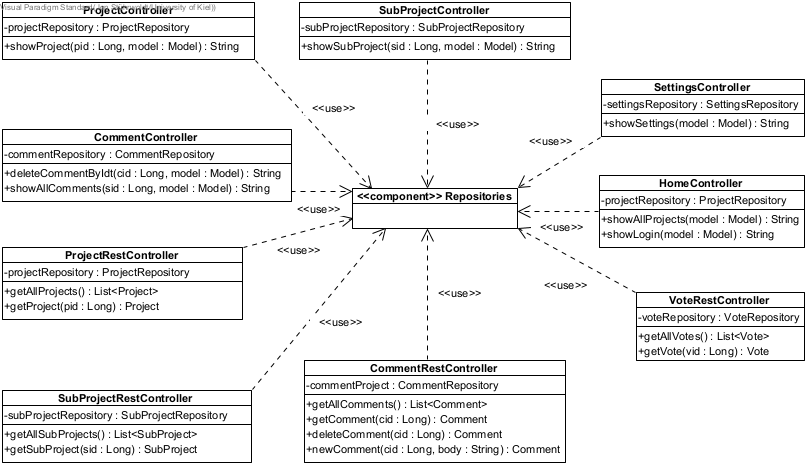
\includegraphics[width=\textwidth]{img/controller.png}	
	\caption{Klassendiagramm - Controller}
	\label{fig:klassendiagramm-cont}
\end{figure}

\begin{table}[H]
	\centering
	\begin{tabularx}{\textwidth}{X X}
		\rowcolor[HTML]{C0C0C0} 
		\textbf{Klassenname} & \textbf{Aufgabe} \\
		HomeController & Klasse, die eine HTML-Seite zurückgibt, die eine Liste aller (Haupt-)Projekte enthält und dem Administrator die Möglichkeit bietet, über einen Button auf die Login-Seite weitergeleitet zu werden. \\
		\rowcolor[HTML]{E7E7E7}
		ProjectController & Klasse, die eine HTML-Seite zurückgibt, welche alle Informationen eines Projektes enthält. Zu diesen Informationen zählt unter anderem eine Liste der zugehörigen Teilprojekte, in der die jeweiligen Seiten der Teilprojekte verinkt sind.  \\
		 SubProjectController &  Klasse, die eine HTML-Seite zurückgibt, die alle Informationen eines Teilprojektes und einen Link zu den Kommentaren dieses Teilprojektes enthält. \\
		 \rowcolor[HTML]{E7E7E7}
		CommentController & Klasse, die eine HTML-Seite zurückgibt, die alle Kommentare eines gegebenen Teilprojektes enthält. Administratoren haben auf dieser Seite außerdem die Möglichkeit Kommentare zu löschen. \\
		SettingsController & Klasse, die eine HTML-Seite zurückgibt, auf welcher Administratoren die System-URLs konfigurieren können.  \\
		\rowcolor[HTML]{E7E7E7}
		ProjectRestController & Klasse, die Methoden für den Austausch von Projekten mit der App über die Rest-API bereitstellt.  \\
		 SubProjectRestController &  Klasse, die Methoden für den Austausch von Teilprojekten mit der App über die Rest-API bereitstellt. \\
		 \rowcolor[HTML]{E7E7E7}
		CommentRestController & Klasse, die Methoden für den Austausch von Kommentaren mit der App über die Rest-API bereitstellt. \\
		VotesRestController & Klasse, die Methoden für den Austausch von Bewertungen/Abstimmungen mit der App über die Rest-API bereitstellt.  \\
	\end{tabularx}
	\caption{Klassenbeschreibung - Web, Controller}
	\label{table:klassenbeschreibung-web-controller}
\end{table}

\section{Klassendiagramm App}

\begin{figure}[H]
	\centering
	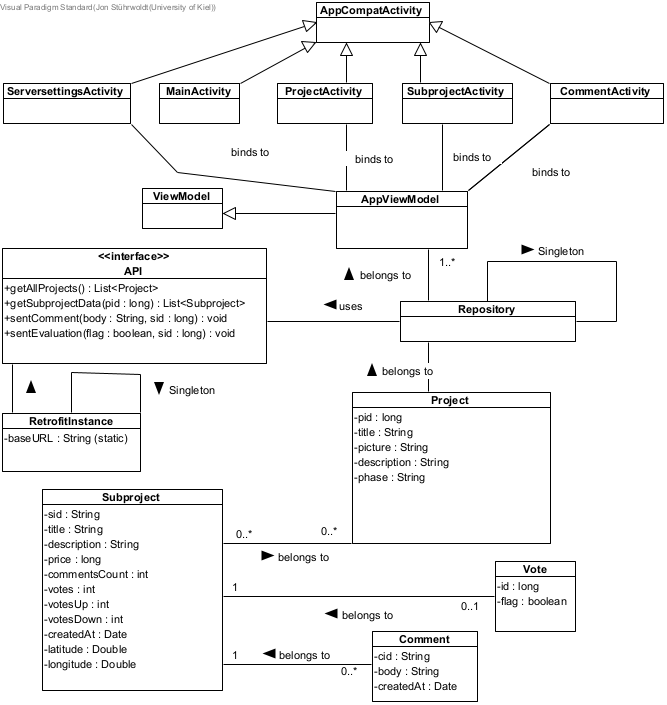
\includegraphics[width=\textwidth]{img/classapp.png}	
	\caption{Klassendiagramm - App}
	\label{fig:klassendiagramm-app}
\end{figure}

\begin{table}[H]
	\centering
	\begin{tabularx}{\textwidth}{X X}
		\rowcolor[HTML]{C0C0C0} 
		\textbf{Klassenname} & \textbf{Aufgabe} \\
		AppCompatActivity &Von Android bereitgestellte Basisklasse für Activities. \\
		\rowcolor[HTML]{E7E7E7}
		MainActivity & Realisiert die Projektübersichtsseite, Startpunkt unserer App. \\
		 Serversettingsactiivity & Realisiert die Server-Einstellungsseite. Hier kann die URL des Backend angepasst werden. \\
		 \rowcolor[HTML]{E7E7E7}
		ProjectActivity & Realisiert die Projektdetailseite und die Auflistung der Teilprojekte. \\
		SubprojectActivity & Realisiert die Teilprojektseite mit einem Kommentareingabebereich.\\
		\rowcolor[HTML]{E7E7E7}
		CommentActivity & Realisiert die Auflistung aller zu dem Teilprojekt geschriebenen Kommentare.  \\
		AppViewModel & Stellt das Bindeglied zwischen View und Model dar.  Verarbeitet die vom Repository erhaltenen Daten und stellt es der View bereit.  \\
		\rowcolor[HTML]{E7E7E7}
		 Viewmodel &  Von Android bereitgestellte Basisklasse für unser AppViewModel. \\
		Repository & Ist für den Datenaustausch zwischen App und Backend zuständig. Die Repository-Klasse tätigt sämtliche API-Calls. \\
		\rowcolor[HTML]{E7E7E7}
		RetrofitInstance & Klasse, um API-Calls mittels http zu realisieren.  \\
		APIService & Benötigtes Interface für Aufrufe an das Backend (nötig für Retrofit).\\
		\rowcolor[HTML]{E7E7E7}
		Project & Klasse für das Projekt.\\
		Subproject & Klasse für das Teilprojekt.\\
		\rowcolor[HTML]{E7E7E7}
		Comment & Klasse für den Kommentar.\\
		Vote & Klasse, die die Evaluierung der Teilprojekte erleichtert.\\
	\end{tabularx}
	\caption{Klassenbeschreibung - App}
	\label{table:klassenbeschreibung-web-controller}
\end{table}
	
	\chapter{Sequenzdiagramme}\label{chp:sequenzdiagramme}
	\thispagestyle{fancy}
	\section{Sequenzdiagramme Web}

%Im Folgendem sind Sequenzdiagramme für elementare Anwendungsfälle gegeben. Sie sollen einen Eindruck bieten, wie für diese die Kommunikation 

\begin{figure}[H]
	\centering
	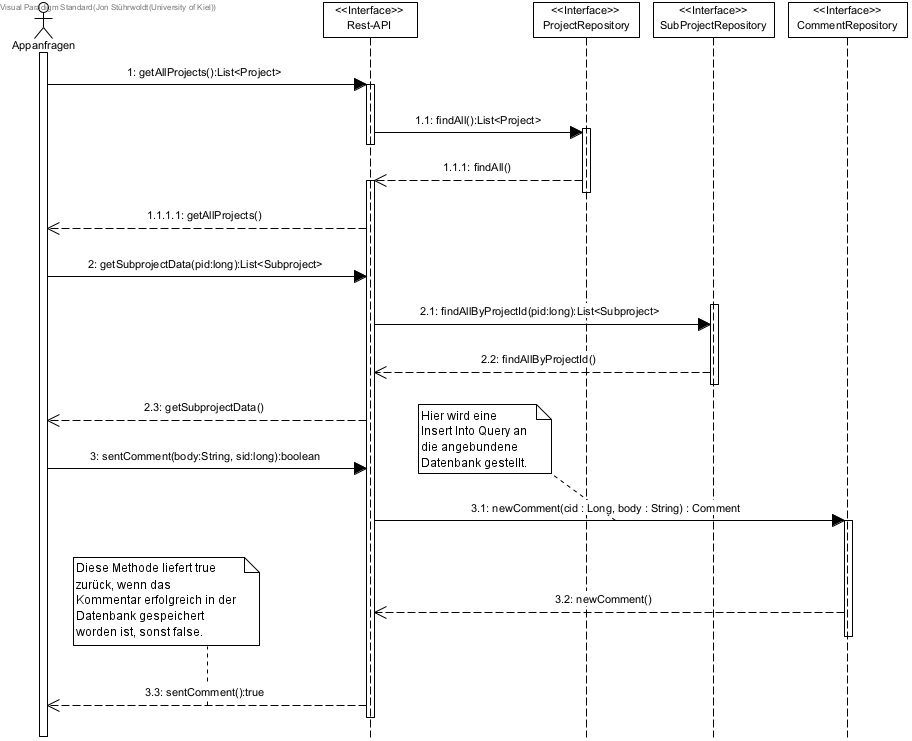
\includegraphics[width=\textwidth]{img/seqwebcreate}		
	\caption{Sequenzdiagramm - Kommentar schreiben}
	\label{fig:sequenz-a}
\end{figure}

Dieses Sequenzdiagramm zeigt den zeitlichen Ablauf des Anwendungsfalles "Kommentar bei Teilprojekt abgeben". Die App fragt hierbei beim Backend
zuerst die Projektdaten, dann die Teilprojektdaten und schließlich die jeweiligen Kommentarlisten der Teilprojekte an. Die einzelnen Anfragen werden
dabei über eine Rest-API geregelt, welches dann im Backend die zur Anfrage gehörigen Daten aus den Repositories abfragt und anschließend wieder an die
App zurücksendet.


\begin{figure}[H]
	\centering
	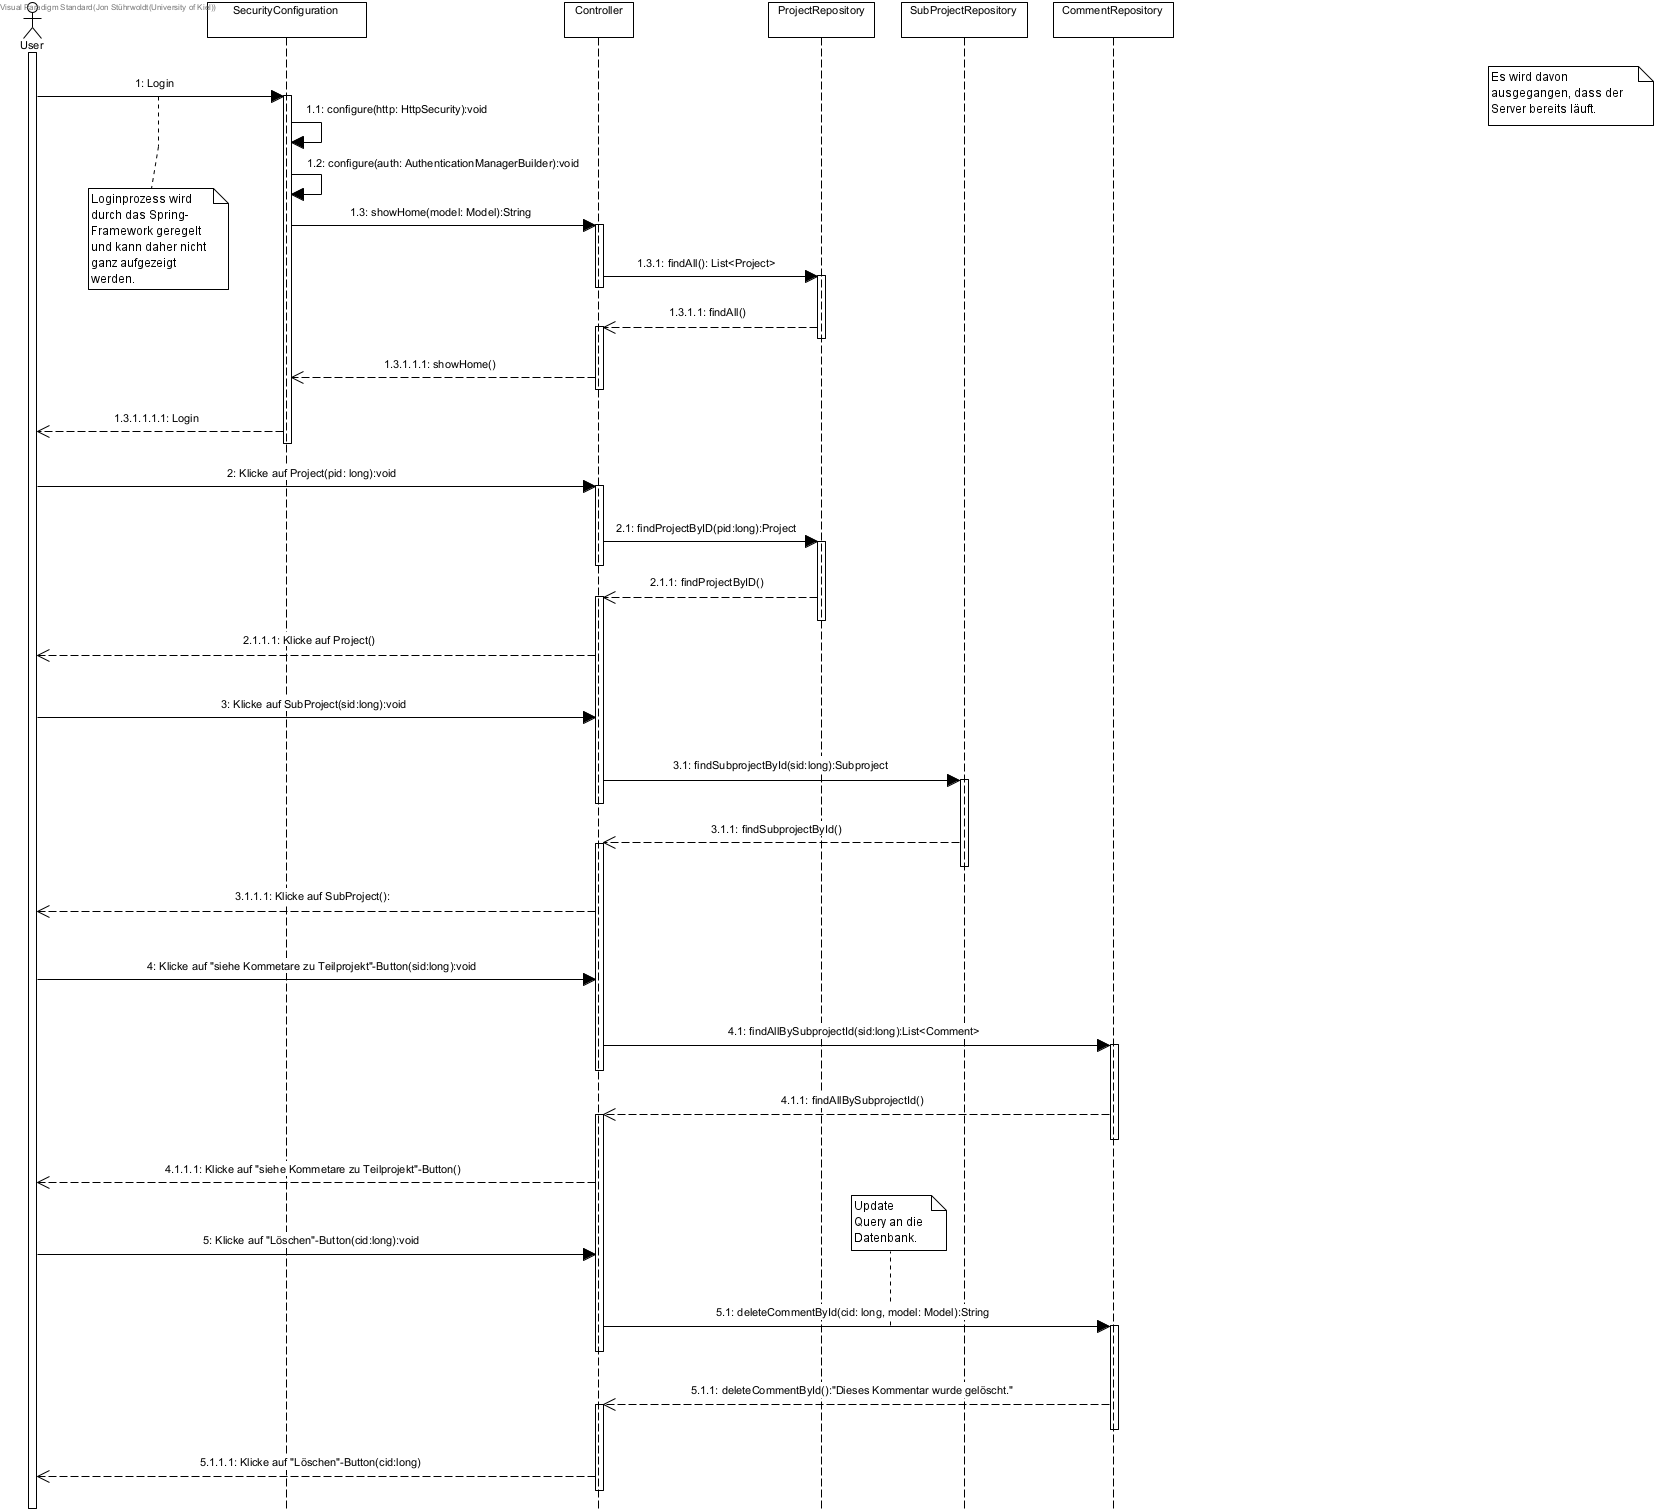
\includegraphics[width=\paperwidth]{img/seqwebdelete}		
	\caption{Sequenzdiagramm - Kommentar löschen}
	\label{fig:sequenz-b}
\end{figure}

Dieses Sequenzdiagramm zeigt den zeitlichen Ablauf des Anwendungsfalles "Kommentar löschen". Um die Berechtigung zu haben, Kommentare löschen zu
können, muss sich der User als Admin einloggen. Der Login-Prozess wird vom Spring Boot Framework übernommen. Nach einem erfolgreichen Login wird
man dann zur ``Home``-Seite weitergeleitet. Dabei wird die Methode showHome() vom Controller aufgerufen, der sich erst die nötigen Daten aus dem
jeweiligen Repository zieht und anschließend eine auf den Daten basierende .html Datei zurückgibt. Der Ablauf vom Controller bis zur .html Datei
geschieht analog mit den Daten vom Projekt, Teilprojekt und Kommentar. 


\section{Sequenzdiagramme App}


\begin{figure}[H]
	\centering
	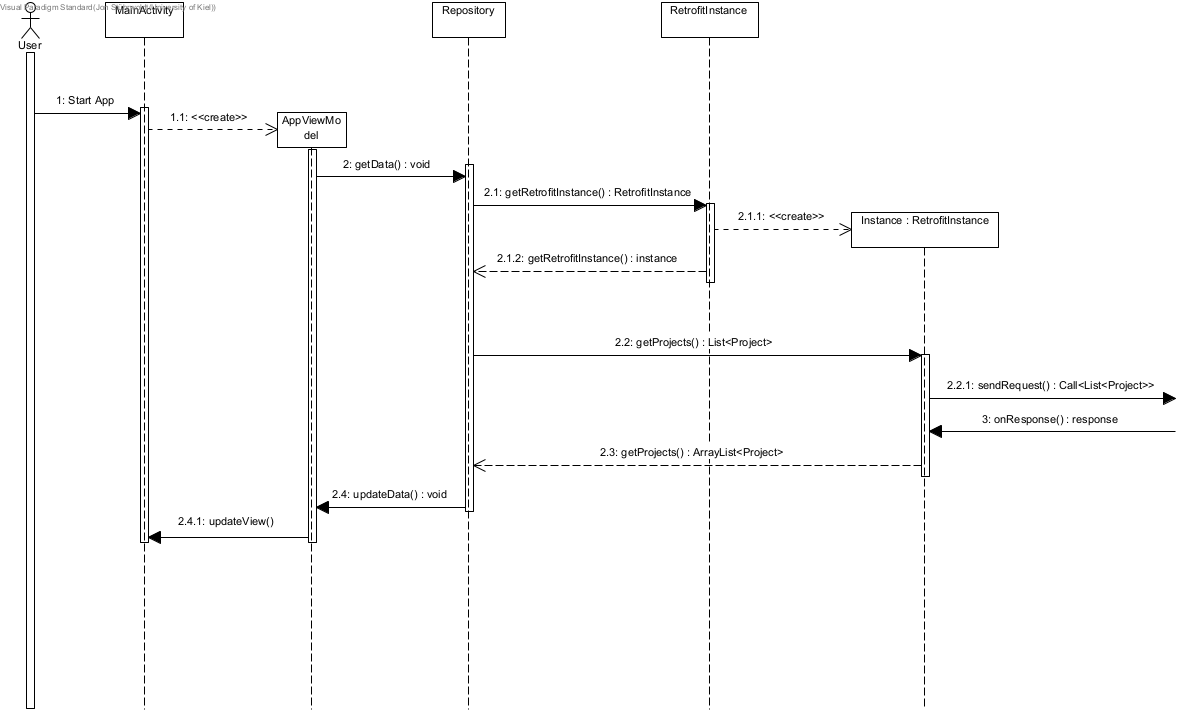
\includegraphics[width=\textwidth]{img/seqappstart}		
	\caption{Sequenzdiagramm - App starten}
	\label{fig:sequenz-c}
\end{figure}

Dieses Sequenz-Diagramm beschreibt den App-Aufruf und das Afragen der Projektdaten über das Backend. Nach dem Start der App initialisiert die MainActivity das AppViewModel. Das AppViewModel stellt eine Anfrage an das Repository. Dort wird eine RetrofitInstance erstellt, über welche die Projektdaten vom Backend abgefragt werden. Die Daten werden zum AppViewModel zurückgegeben und auf der MainActivity dargestellt.


\begin{figure}[H]
	\centering
	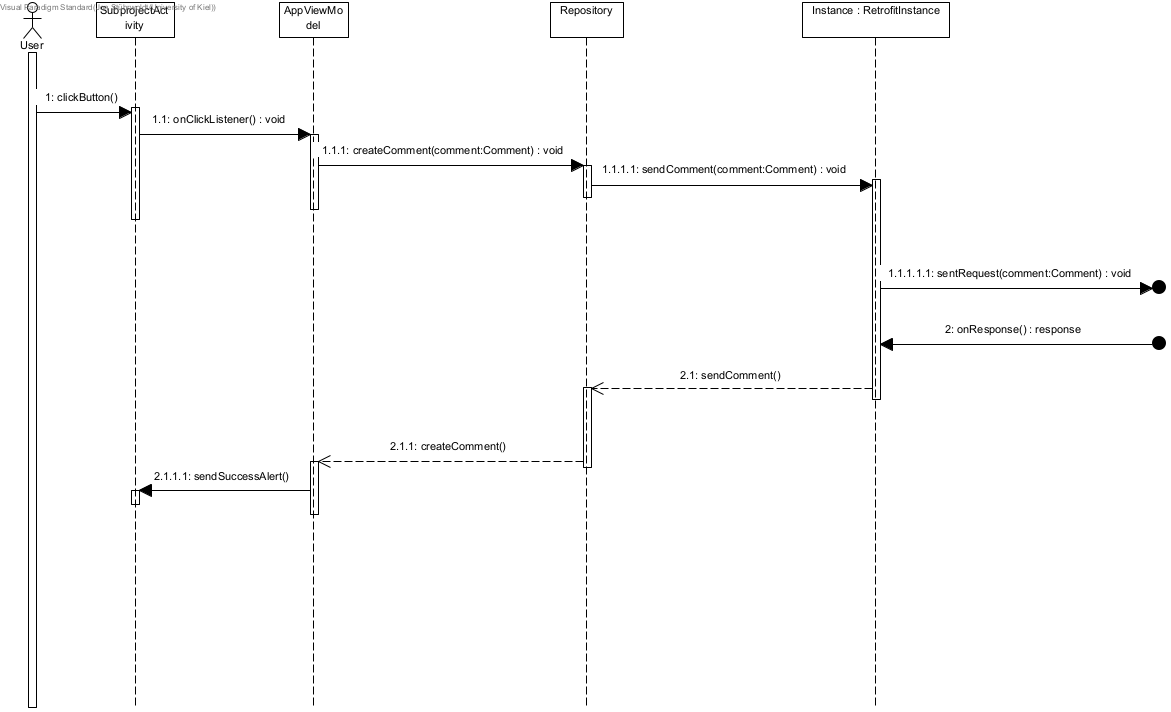
\includegraphics[width=\textwidth]{img/seqappcreate}		
	\caption{Sequenzdiagramm - Kommentar schreiben}
	\label{fig:sequenz-d}
\end{figure}

Die Abbildung zeigt das Sequenz-Diagramm zum Hinzufügen eines neuen Kommentars zu einem Teilprojekt. Nach dem Eingeben des Kommentars kann er über einen Button die Eingabe bestätigen. Dabei ruft das AppViewModel eine Methode zum Erstellen eines neuen Kommentars im Repository auf. Das Repository leitet den Kommentar weiter an das Backend. Im Anschluss wird eine Success-Message an den Benutzer zurückgegeben. 
	
	%\bibliography{references}
	%\pagenumbering{gobble} % Nummerierung deaktivieren
	
\end{document}
